\begin{problem}{Conga line}{standard input}{standard output}{3 seconds}

Conga is a traditional dance in which people make a line, grab each other by the waist and start dancing around.

You are at a party and your favorite Conga song starts playing. Since you want to make the most of it, you'd like to organize everybody and start dancing as soon as possible.

The dance floor is modeled as an infinite straight line with people standing on positive integer coordinates. There is at most one person at each point.
Every second, a person can move one unit to the left or one unit to the right, as long as no one else is standing there. However, since
it's a crazy party and people are already drunk, at most one person can move every second (in other words, no two people can move simultaneously).

Nobody will start dancing until everybody is organized in a perfect line. You want to find the minimum amount of time it takes to start dancing, i.e. the time it takes to make people stand in such a way that there are no empty spaces between them.

For example, imagine there are 4 people at the party, standing at positions 2, 4, 5 and 8:

\begin{center}
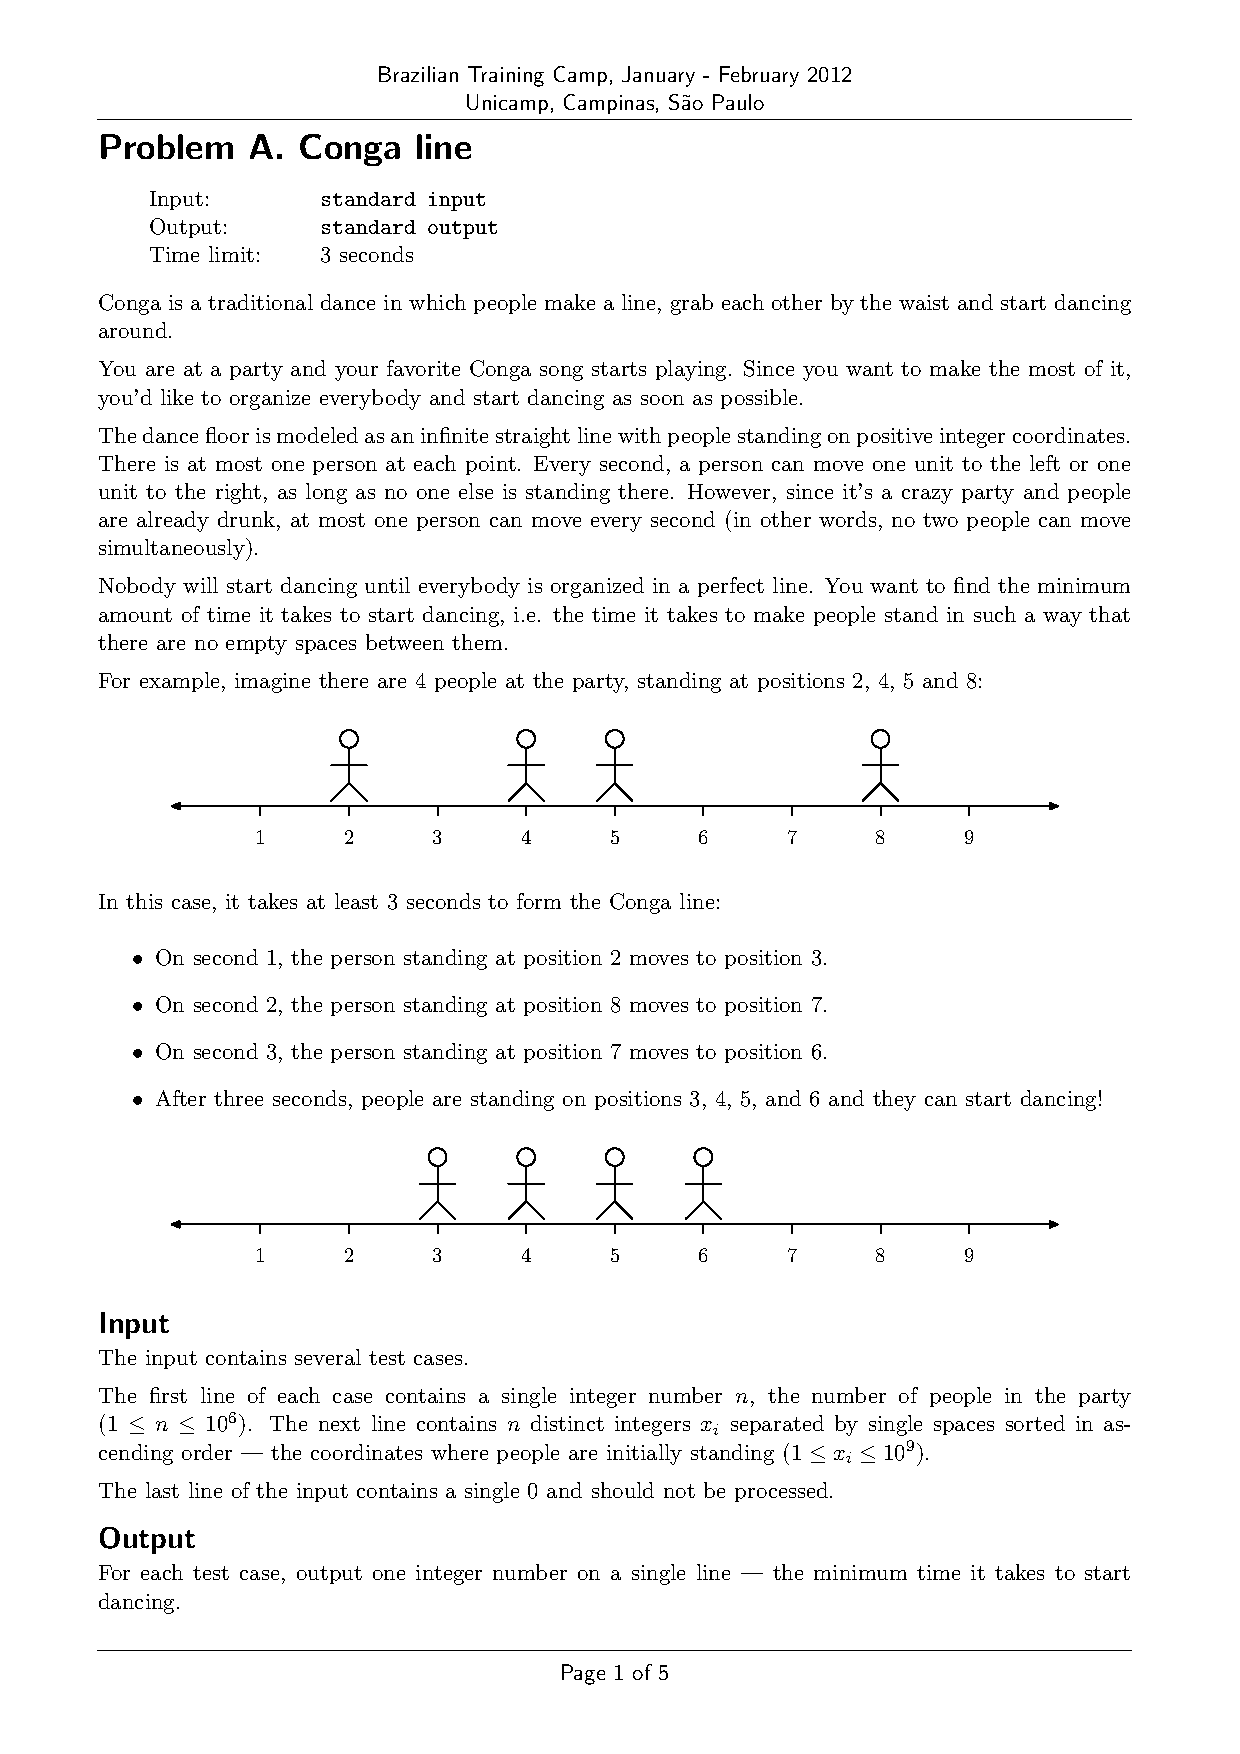
\includegraphics{pics/conga.1}
\end{center}


In this case, it takes at least 3 seconds to form the Conga line:
\begin{itemize}
  \item On second 1, the person standing at position 2 moves to position 3.
  \item On second 2, the person standing at position 8 moves to position 7.
  \item On second 3, the person standing at position 7 moves to position 6.
  \item After three seconds, people are standing on positions 3, 4, 5, and 6 and they can start dancing!
\end{itemize}

\begin{center}
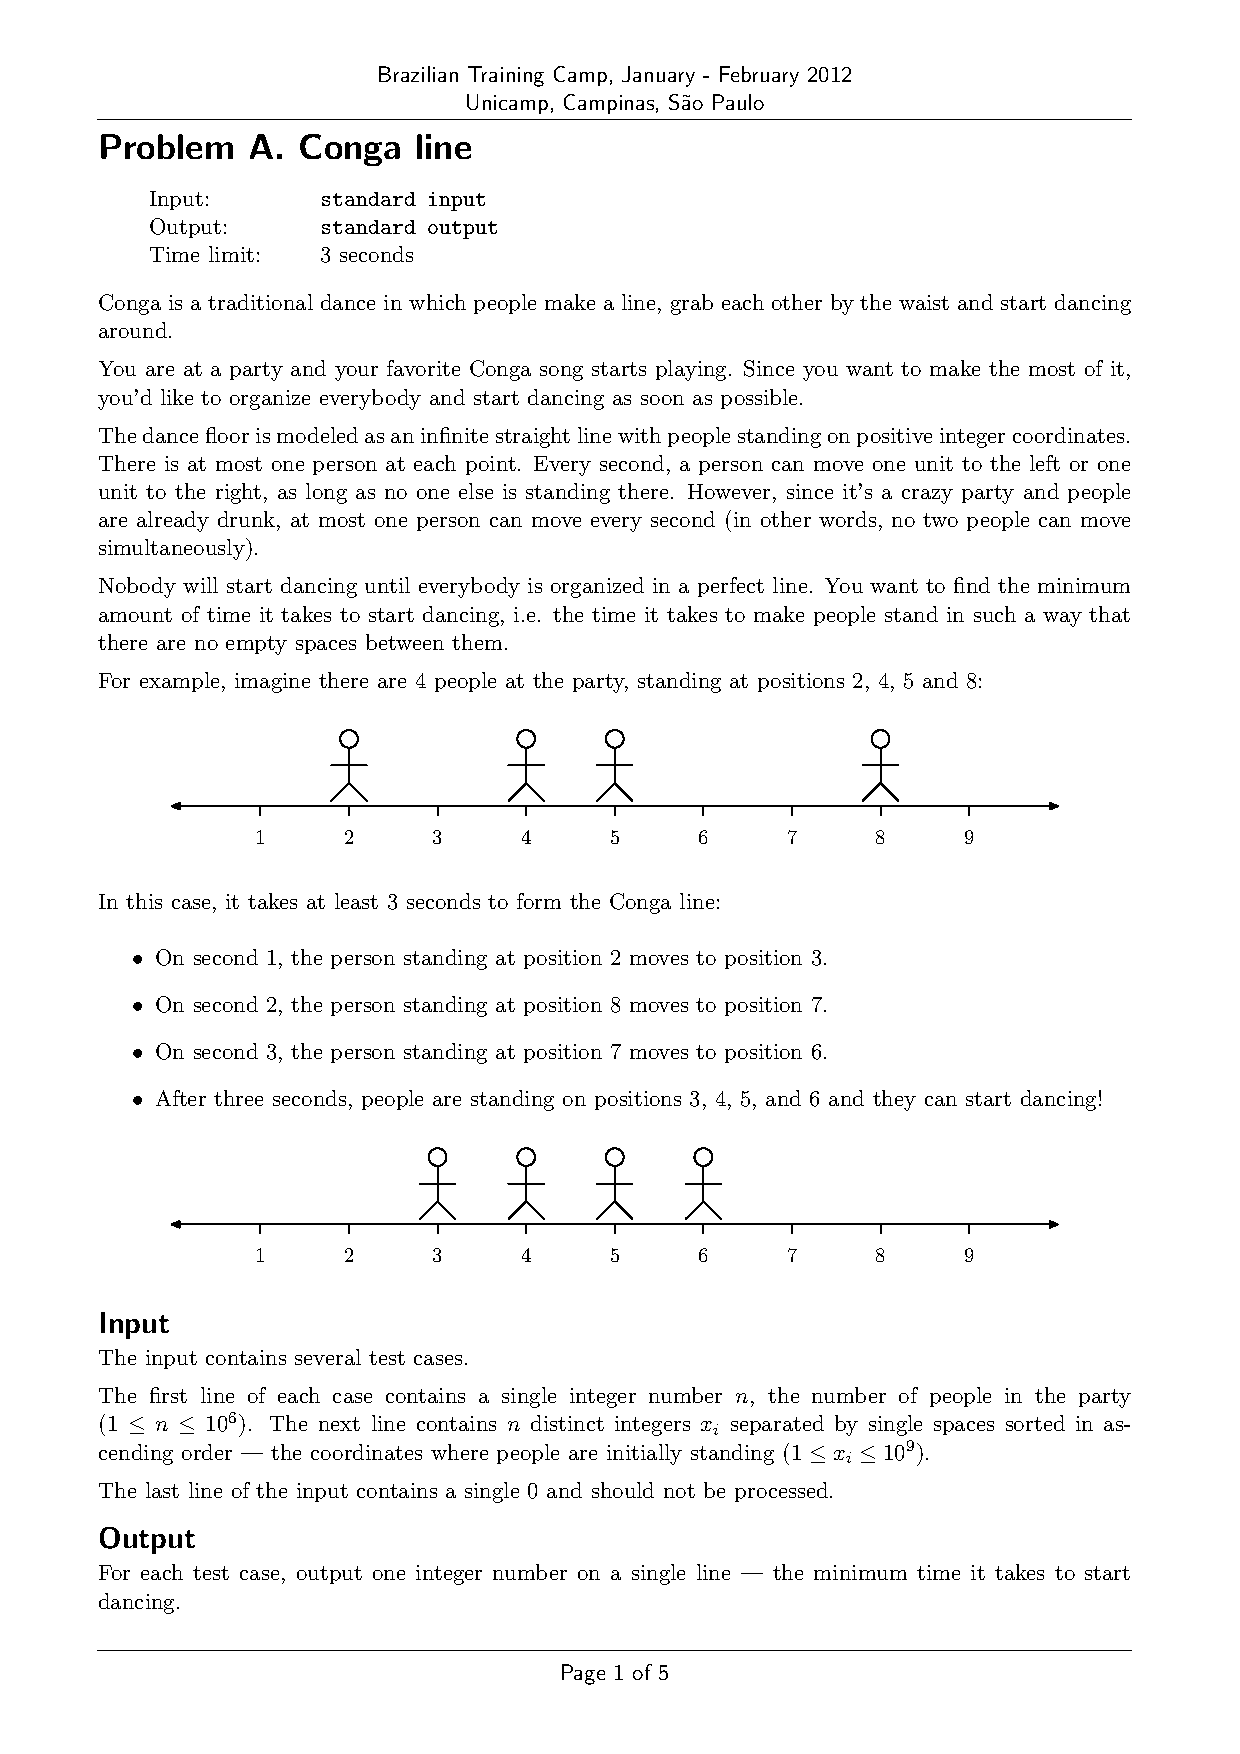
\includegraphics{pics/conga.2}
\end{center}


\InputFile

The input contains several test cases.

The first line of each case contains a single integer number $n$, the number of people in the party ($1 \le n \le 10^6 $).
The next line contains $n$ distinct integers $x_i$ separated by single spaces sorted in ascending order --- the coordinates where people are initially standing 
($1 \le x_i \le 10^9$).

The last line of the input contains a single $0$ and should not be processed.

\OutputFile

For each test case, output one integer number on a single line --- the minimum time it takes to start dancing.

\Example

\begin{example}
\exmp{
4
2 4 5 8
1
10
4
20 24 25 26
2
1 2
2
1 1000000000
0
}{
3
0
3
0
999999998
}%
\end{example}

\end{problem}
